\section{Quick reminder - What is the SpaceAPI?}

\begin{frame}[c]{What is the SpaceAPI}
    \begin{itemize}
        \item A JSON schema
        \item Describes your hackerspace
        \item Mostly static but may contain dynamic data
    \end{itemize}
\end{frame}

\begin{frame}[fragile]{SpaceAPI Excerpt}
    \begin{minted}[fontsize=\footnotesize]{json}
{
    "api": "0.13",
    "contact": {
        "email": "vorstand@lists.coredump.ch",
        "twitter": "@coredump_ch"
    },
    "sensors": {
        "people_now_present": [
            {
                "location": "Hackerspace",
                "value": 0
            }
        ]
    },
    "state": {
        "message": "Open Mondays from 20:00",
        "open": false
    }
}
    \end{minted}
\end{frame}

\section{The Beginning}

\begin{frame}[c]{Requirement}
    \begin{itemize}
        \item Serve SpaceAPI JSON data
        \item Mostly static except state and sensors
        \item Endpoint to update sensor data
    \end{itemize}
\end{frame}

\begin{frame}[c]{A 100 Line Python Script}
    \begin{itemize}
        \item Our first implementation was \~100 lines of Python\footnote{\url{https://github.com/coredump-ch/status/tree/1ae92a58c13b5ee106671092717f1bf4b4b9ee97}}
        \item Hacky but worked
    \end{itemize}
\end{frame}

\begin{frame}[c]{A 100 Line Python Script}
    \centering
    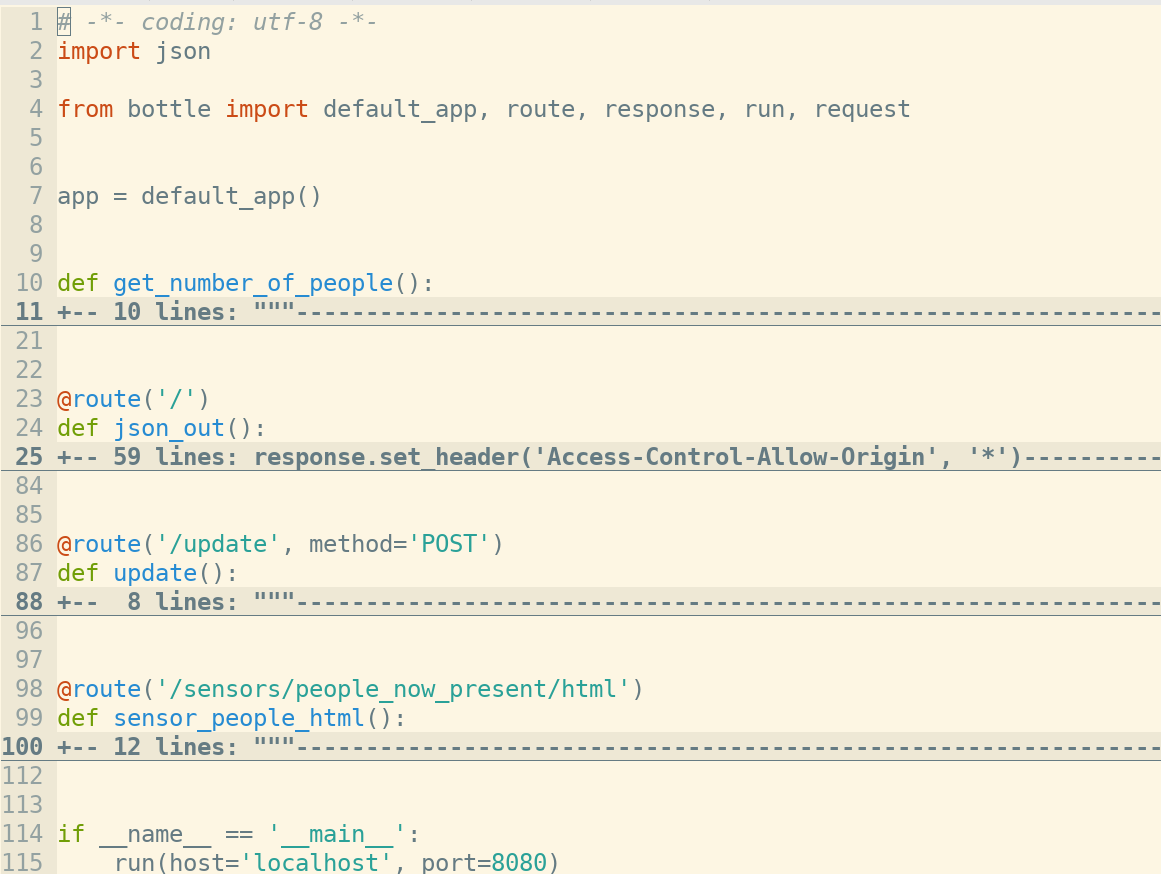
\includegraphics[height=0.98\textheight]{./spaceapi_in_rust/python2.png}
\end{frame}

\begin{frame}[fragile]{Reading the sensor...}
    \begin{minted}{python}
def get_number_of_people():
    """
    Return an integer or None.
    """
    people = None
    try:
        with open('people.txt', 'r') as f:
            people = int(f.read().strip())
    except:
        pass
    return people
    \end{minted}
\end{frame}

\begin{frame}[fragile]{Updating the sensor...}
    \begin{minted}{python}
@route('/update', method='POST')
def update():
    """
    Update the data in a text file.
    TODO: Public / Private key crypto.
    """
    people = int(request.POST.get('people'))
    with open('people.txt', 'w') as f:
        f.write(str(people))
    return 'OK'
    \end{minted}
\end{frame}

\begin{frame}[c]{Hacky, but actually worked!}
    \begin{itemize}
        \item Hacky but worked
        \item Probably a race conditions with the file access?
        \item Ugly to extend with further sensors
    \end{itemize}
\end{frame}

\section{Rewrite it in Rust!}

\begin{frame}[c]{Why?}
    \begin{itemize}
        \item If it worked why rewrite it?
        \pause\item Learn Rust
        \item Have a reasonable sized project
    \end{itemize}
\end{frame}

\begin{frame}[c]{Overengineer it!}
    \centering
    
\includegraphics[height=0.8\textheight]{./spaceapi_in_rust/overengineer_all_the_things.jpg}
\end{frame}

\begin{frame}[c]{Goals}
    \begin{itemize}
        \item Encode the SpaceAPI rules in the type system \\
            $\rightarrow$ Impossible to generate non conforming JSON
        \item Use a better backend for data storage
        \item Make it reusable for other hackerspaces
    \end{itemize}
\end{frame}
